% !TeX root = ../main.tex

\section{Density Estimation}
Let $p(\vec{x})$ denote a probability density function pdf then:

\begin{enumerate}
  \item $p(\vec{x}) \ge 0$
  \item $\int_{-\infty}^\infty p(\vec{x}) \,d\vec{x} = 1$
  \item $p(\vec{a} \le \vec{x} \le \vec{b}) = \int_{\vec{a}}^{\vec{b}} p(\vec{x}) \,d\vec{x}$
\end{enumerate}

The task of density estimation is to obtain a continous representation of the underlying pdf from a set of discrete samples (massumants). Note: that if we have the pdf we can do statistical analysis.

\subparagraph{Parametric density estimation}
(mostly Pattern Recognition)

Make an assumption about the underlying distribution (e.g. Gausian, GMM) and determine the best fitting distribution parameters from the data. (ML estimation, MAP estimation)

\subparagraph{Non-parametric density estimation}

We make no assumption of the underlying Model.

\subsection{Parzen-Rosenblatt estimator}
???Idea: Quantify the number of samples with a window

\begin{figure}[H]
  \centering
  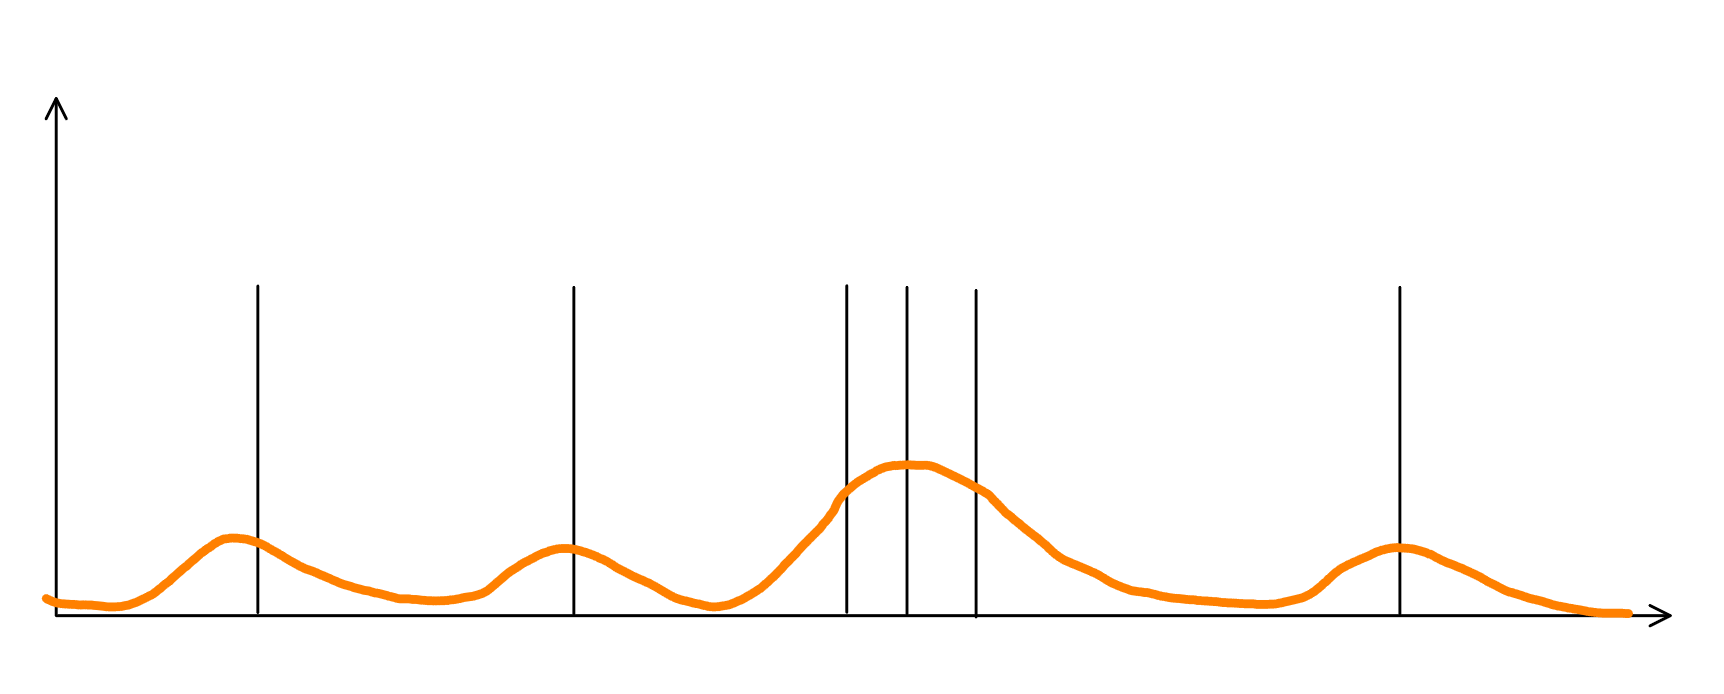
\includegraphics[width=0.8\textwidth]{01-pr-estimator}
  \caption{A PDF describing the distribution of measurements}
\end{figure}

The Parzen window estimator interpolates the pdf from the observations in the neighbourhood of a position $x$, using an appropriate kernel/window function.

\subparagraph{Short derivtion:}
Let $p_R$ denote the probability that $\vec{x}$ lies within region $R$:

\begin{equation*}
  p_R = \int_R p(\vec{x}) \,d\vec{x}
\end{equation*}

Now assume that $p(\vec{x})$ is approximately constant in R.

\begin{equation*}
  p_R \approx p(\vec{x}) \int_R \,d\vec{x}
\end{equation*}

For example, let $R$ be a d-dimensional hypercube with side length $h$, then its volume\footnote{$\int_R \,d\vec{x}$ is just the volume of $R$}\footnote{We also write $V_R$ for the volume} is $h^d$

\begin{equation*}
  p_R \approx p(\vec{x}) V_R
\end{equation*}

Let $p_R = \dfrac{k_R}{N}$, we determine the probability of making observations in region $R$ by counting the samples in $R$ ($=k_R$) and dividing by the total number of samples. Note: $p_R$ is also called the ``relative frequency''

\begin{equation*}
  p(\vec{x}) = \dfrac{p_R}{V_R} = \dfrac{k_R}{V_R N}
\end{equation*}

Let's write the parzen window estimator as a function of a kernel\footnote{Omit $h^d$ if the kernel is gaussian} $k(\vec{x}; \vec{x_i})$, then

\begin{equation*}
  p(\vec{x}) = \dfrac{1}{h^d N} \sum_{i=1}^N k(\vec{x}; \vec{x_i})
\end{equation*}

where\footnote{$\vec{x_i}$ and $\vec{x}$ are not father apart then $0.5 h$ in any dimension $k$}

\begin{equation*}
  k(\vec{x}; \vec{x_i}) = \begin{cases}
    1 &\text{when } \dfrac{|x_{i,k} - x_k|}{h} \le \dfrac{1}{2}\\
    0 &\text{otherwise}
  \end{cases}
\end{equation*}

equivalently, if we use a (multivariate) gaussian kernel:


\begin{equation*}
   k(\vec{x}; \vec{x_i}) = \dfrac{1}{{(2\pi)}^d |\Sigma|} e^{-{(\vec{x} - \vec{x_i})}^T \Sigma^{-1}(\vec{x}-\vec{x_i})}
\end{equation*}

\subparagraph{A note on applications}
\begin{itemize}
  \item General remark: We obtain a continuous pdf, i.e.\ desity estimation converts a list of measurments to a statistical model
  \item Specific example: We can sample from a pdf. This means that we have a princeple way of generating new / more / \ldots{} data that behaves / looks / \ldots{} similary to the observations.
\end{itemize}

\subparagraph{Q:} How can we (practically) sample from a pdf?

\begin{figure}[H]
  \centering
  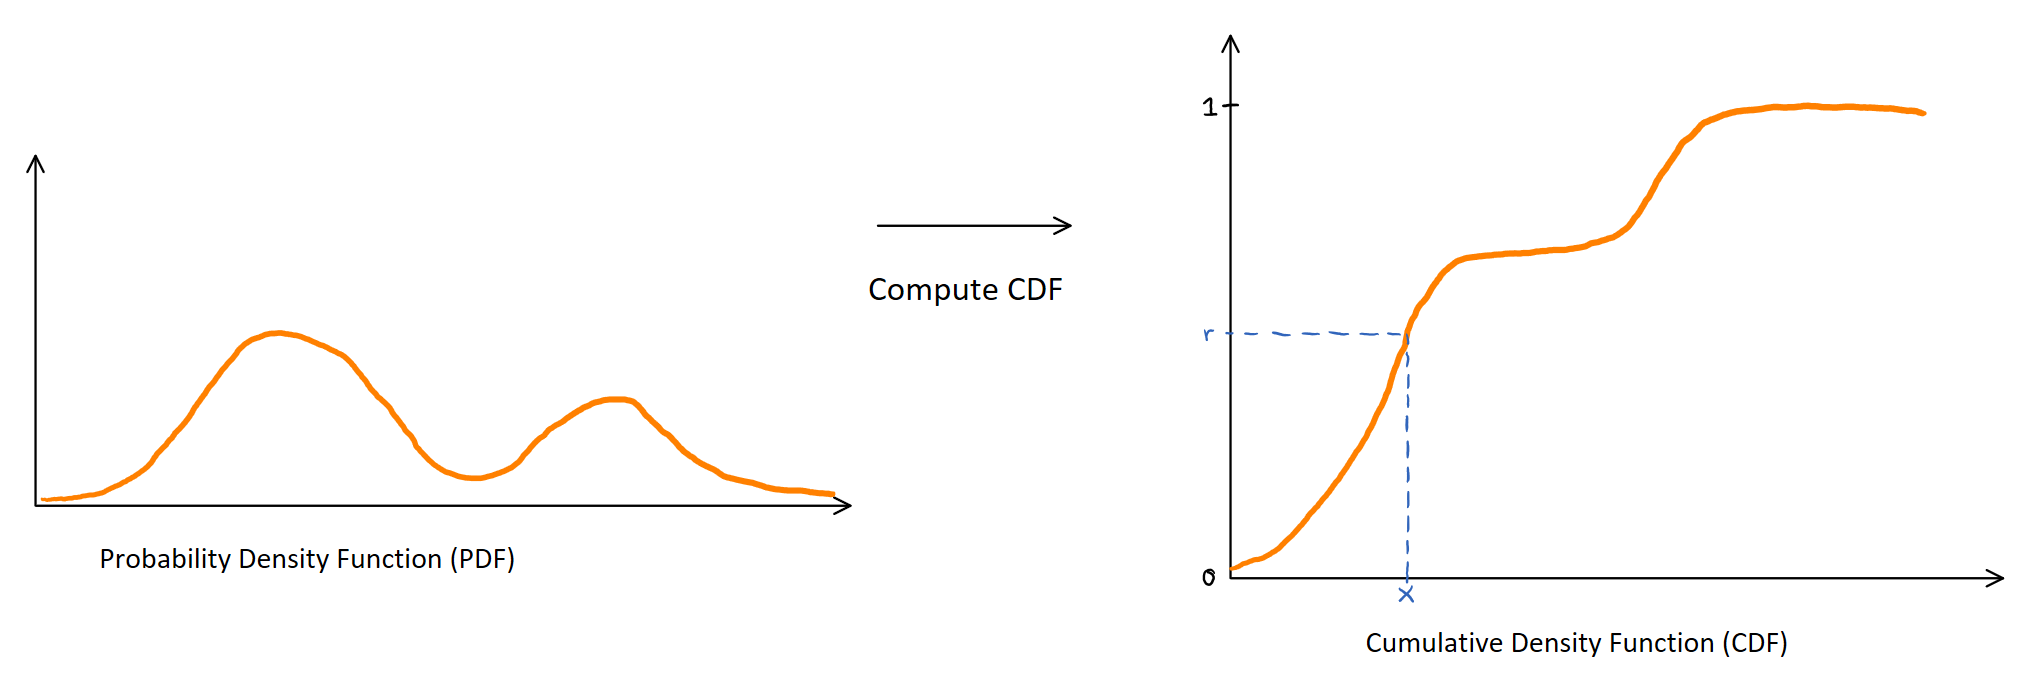
\includegraphics[width=\textwidth]{02-pdf-cdf}
\end{figure}

Compute through discretisation of the pdf $cdf[i] = cdf[i-1] + pdf[i]$. Then draw a uniformly distributed number ($r$) between 0 and 1. The sampled value is $x$ where $cdf[x] = r$


\subparagraph{Q:} How can we determine a good window / kernel width h?

Let's do ML est.\ with a cross-vaslidation (cv) (e.g.\ leave-one-sample-out cv)

\begin{equation*}
  p_{h,N-1}^j(\vec{x}) = \dfrac{1}{h^d N} \sum_{i=1 (i \neq j)}^N k(\vec{x}; \vec{x_i})
\end{equation*}

We estimate the pdf from all samples except $\vec{x_j}$. $\vec{x_i}$ will be used to evaluate the quality of the pdf using window siye h.

\subparagraph{Q:} How do the results change with varing window size?

\begin{figure}[H]
  \centering
  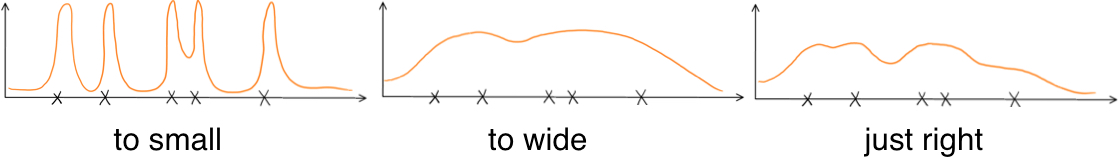
\includegraphics[width=0.8\textwidth]{03-window-size}
\end{figure}

\begin{equation*}
\hat{h} = \argmax_h L(h) = \argmax_h \prod_{j=1}^N p_{h,N-1}^j(\vec{x_j}) = \argmax_h \sum_{j=1}^N \log p_{h,N-1}^j(\vec{x_j})
\end{equation*}

The position of the maximum does not change, because the logarithm is a strictly monotonic function.
